
\chapter{Tunneldiode\label{chapter:tunneldiode}}
\lhead{Tunneldiode}
\begin{refsection}
\chapterauthor{Stefan Hedinger}

\section{Leitmechanismen von Halbleiterdioden}
\rhead{Leitmechanismen von Halbleiterdioden}

Die Tunneldiode ist ein nicht sehr h"aufig verwendetes, aktives und dynamisches Halbleiterelement.
Als Halbleitermaterial wird f"ur ihren  Aufbau Germanium verwendet. 
Um die Tunneldiode und ihren Aufbau besser erkl"aren zu k"onnen, ziehen wir zum Vergleich eine normale Germaniumdiode heran. 
Der Aufbau einer Diode besteht im wesentlichen aus einer positiv und einer negativ dotierten Seite, dem sogenannten p-n-"Ubergang. 
Dazwischen befindet sich die Sperrzone, welche man auch als Potentialbarriere betrachten kann.

\begin{figure}	%Bild Bändermodell Germaniumdiode Vf = 0
\centering
\includegraphics[width=0.5\textwidth]{tunneldiode/tunnel-9.pdf}
\caption{B"andermodell der Germaniumdiode mit $V_F = 0$
\label{tunnel:BaendermodellG0}}
\end{figure}

Ohne Vorw"artsspannung sind die Energieniveaus wie in Abbildung~\ref{tunnel:BaendermodellG0} verteilt. 
Das Ferminivau $E_F$ ist in p und n auf derselben H"ohe.
Oberhalb des Ferminiveaus sind fast keine bewegliche Elektronen vorhanden.
Das Leitungsband $E_C$ ist "uber dem Ferminiveau  und das Valenzband $E_V$ unter dem Ferminiveau. 
Solange die Energie der Elektronen kleiner als das Potential der Barriere ist, leitet die Diode nicht.
Den Elektronen kann mit der Vorw"artsspannung Energie von aussen zugef"uhrt werden.

\begin{figure}	%Bild Bändermodell Germaniumdiode Vf > 0
\centering
\includegraphics[width=0.5\textwidth]{tunneldiode/tunnel-11.pdf}
\caption{B"andermodell der Germaniumdiode mit $V_F > 0$
\label{tunnel:BaendermodellG}}
\end{figure}

Legt man eine positive Spannung in Vorw"artsrichtung an, hebt man damit die Energie der Elektronen an. 
Wie in Abbildung~\ref{tunnel:BaendermodellG} ersichtlich, wird auch das Ferminiveau auf der n-Seite gr"osser als auf der p-Seite. 
Bei etwa 200mV Vorw"artsspannung beginnt die Germaniumdiode zu leiten. 
Zum Vergleich wurden zwei verschiedene Typen Germaniumdioden vermessen. 
In Abbildung~\ref{tunnel:Germaniumdioden} ist der Vorw"artsstrom durch die Diode in Abh"angigkeit zur Vorw"artsspannung aufgetragen.

\begin{figure}	%Bild Kennlinie der Germaniumdioden
\centering
\includegraphics[width=0.7\textwidth]{tunneldiode/tunnel-6.pdf}
\caption{Kennlinien von zwei verschiedenen Germaniumdiodentypen
\label{tunnel:Germaniumdioden}}
\end{figure}

Die Tunneldiode unterscheidet sich im Vergleich zur Germaniumdiode in zwei Punkten. 
Zum einen ist die Dotierung des p-n-"Ubergangs gr"osser, zum anderen die Sperrschicht viel d"unner. 
Diese beiden Unterschiede erm"oglichen den Tunneleffekt.

Das B"andermodell der Tunneldiode ist fast identisch mit dem der Germaniumdiode. 
Auch hier ist das Ferminiveau ohne Vorw"artsspannung auf derselben H"ohe. 
Wie in Abbildung~\ref{tunnel:Baendermodell0} ersichtlich, ist auf der p-Seite sowohl das Valenzband als auch das Leitungsband "uber dem Ferminiveau. 
Auf der n-Seite ist es genau umgekehrt, da sind beide B"ander unter dem Ferminiveau.
Der Grund daf"ur ist folgender.
Durch die starke Dotierung werden zus"atzliche Elektronen eingebracht.
Diese Elektronen sind "uberz"ahlig und stehen somit als Leitungselektronen zur Verf"ugung.
Darum reicht jetzt das Leitungsband unter das Ferminiveau.
Liegt keine Vorw"artsspannung an, tunneln etwa gleich viele Elektronen von den zwei Richtungen durch die Barriere.
Somit haben wir keinen Strom der fliesst, da sich die St"ome genau aufheben.
Sobald wir eine kleine positive Vorw"artsspannung anlegen, "uberwiegen die in Durchlassrichtung tunnelnden Elektronen.
Es fliesst also ein Strom.
Die Diode beginnt zu leiten, obwohl die Elektronen nicht "uber die Potentialbarriere r"uber k"onnen. 
Sie tunneln durch die Barriere hindurch.
Erh"ohen wir die Vorw"artsspannung weiter, verschieben sich die Energieniveaus 
Die Abbildung ~\ref{tunnel:Baendermodellmax} zeigt die gr"osste "Uberlappung. 
In diesem Fall wird auch der Tunnelstrom maximal. 
In Abbildung ~\ref{tunnel:Baendermodellmin} wird die "Uberlappung wieder kleiner. 
Die Folge davon ist, dass der Tunnelstrom ebenfalls wieder abnimmt.
Sobald aber die Vorw"artsspannung gen"ugend hoch ist, und somit auch das Potential der Elektronen, setzt die normale Diodenleitung ein.

\begin{figure}	%Bild Bändermodell Tunneldiode Vf = 0
\centering
\includegraphics[width=0.5\textwidth]{tunneldiode/tunnel-10.pdf}
\caption{B"andermodell der Tunneldiode mit $V_F = 0$
\label{tunnel:Baendermodell0}}
\end{figure}

\begin{figure}	%Bild Bändermodell Tunneldiode IT = max
\centering
\includegraphics[width=0.5\textwidth]{tunneldiode/tunnel-12.pdf}
\caption{B"andermodell der Tunneldiode mit maximalem Tunnelstrom
\label{tunnel:Baendermodellmax}}
\end{figure}

\begin{figure}	%Bild Bändermodell Tunneldiode IT abnehmend
\centering
\includegraphics[width=0.5\textwidth]{tunneldiode/tunnel-13.pdf}
\caption{B"andermodell der Tunneldiode mit $V_F > 0$, kein Tunnelstrom
\label{tunnel:Baendermodellmin}}
\end{figure}

Die spezielle Kennlinie der Tunneldiode ist in der Abbildung~\ref{tunnel:Tunneldiode} ersichtlich.

\begin{figure}	%Bild Kennlinien der Tunneldiode und GE-Dioden
\centering
\includegraphics[width=0.7\textwidth]{tunneldiode/tunnel-5.pdf}
\caption{Blau: spezielle Kennlinie der Tunneldioden. Rot: Kennlinien von normalen Germaniumdioden.
\label{tunnel:Tunneldiode}}
\end{figure}

\section{Quantenmechanische Berechnung des Tunneleffektes}
\rhead{Quantenmechanische Berechnung des Tunneleffektes}
Als Modell f"ur die bei der Tunneldiode beobachtete Leitung bei geringer Spannung betrachten wir das Potential
\[
V(x)=\begin{cases}
V_0& \qquad \text{wenn } x \in [-a,a]\\
0&   \qquad \text{sonst}
\end{cases}
\]
in den verschiedenen Bereichen.

Damit ein Strom fliessen kann, muss ein Ladungstr"ager, welcher von links kommt, nach rechts gelangen k"onnen. 
Die Energie des einfallenden Teilchens ist $E$ und es gilt
\[
0 < E < V_0.
\]
In der Mitte ist aber eine Barriere, welche ein h"oheres Potential als das Teilchen selber aufweist. 
In der klassischen Mechanik ist klar, dass dieses Teilchen nicht von links nach rechts kommt sondern an der Barriere bei $-a$ reflektiert wird. 
In der Quantenmechanik k"onnen Teilchen jedoch durch die Barriere durchtunneln. (Abbildung~\ref{tunnel:Potentialbarriere})

\begin{figure}	%Bild Kastenpotential
\centering
\includegraphics[width=0.7\textwidth]{tunneldiode/tunnel-4.pdf}
\caption{Visualisierung der Potentialbarriere
\label{tunnel:Potentialbarriere}}
\end{figure}

Die nachfolgenden Berechnungen sollen helfen, den Tunneleffekt zu verstehen.  
Als erstes betrachten wir die station"are Schr"odingergleichung f"ur die Wellenfunktion $\Phi(x)$. 
Dabei ist $m$ die Masse und $E$ die Energie des Teilchens.
\[
E\Phi(x) = -\frac{\hbar^2}{2m}\frac{d^2}{dx^2}\Phi(x) + V(x)\Phi(x)
\]
Im Bereich \textrm{I} und \textrm{III} verwenden wir f"ur die Wellenfunktion den allgemeinen Ansatz
\[
\Phi(x) = Ae^{ikx}+Be^{-ikx}.
\]
F"ur $k$ gilt dabei
\[
k = \sqrt{\frac{2mE}{\hbar^2}}.
\]
Der Koeffizient $A$ steht in beiden Bereichen f"ur die einlaufende Welle, $B$ f"ur die reflektierte Welle.

F"ur die Wellenfunktion im Bereich \textrm{II} lautet die Gleichung
\[
\Phi_\text{II}(x) = \alpha e^{\kappa x} + \beta e^{-\kappa x}
\]
da wir in der Potentialbarriere einen exponentiellen Abfall oder Anstieg erwarten. 
$\kappa$ ist
\[
\kappa = \sqrt{\frac{2m}{\hbar^2}(V_0 - E)}.
\]
Insgesamt haben wir nun sechs Unbekannte. 
Im Bereich \textrm{I} die Koeffizienten $A_1$ und $B_1$, im Bereich \textrm{II} $\alpha$ und $\beta$ und im Bereich \textrm{III} $A_2$ und $B_2$. 
Damit die Wellenfunktion ohne Spr"unge zusammengesetzt werden kann, muss
\begin{equation}
\Phi_\text{I}(-a) = \Phi_\text{II}(-a)
\label{tunnel:fktwert-a}
\end{equation}
\begin{equation}
\Phi_\text{II}(a) = \Phi_\text{III}(a)
\label{tunnel:fktwerta}
\end{equation}
\begin{equation}
\Phi_\text{I}'(-a) = \Phi_\text{II}'(-a)
\label{tunnel:steigung-a}
\end{equation}
\begin{equation}
\Phi_\text{II}'(a) = \Phi_\text{III}'(a)
\label{tunnel:steigunga}
\end{equation}
gelten.
Somit haben wir ein Gleichungssystem mit vier Gleichungen f"ur sechs Unbekannte.
Wir brauchen also die Ableitungen der allgemeinen Wellenfunktionen.
\[
\Phi_\text{I}'(x) = Aike^{ikx} - Bike^{-ikx}
\]
\[
\Phi_\text{II}'(x) = \alpha \kappa e^{\kappa x} - \beta \kappa e^{-\kappa x}
\]
Wir rechnen ab hier mit Matrizen weiter. 
Dies hat den Vorteil, dass sich gewisse Terme vereinfachen lassen. 
Auch mit der Matrizenrechnung ist es nicht m"oglich alle sechs Unbekannten zu bestimmen. 
Es ist aber m"oglich das Verh"altnis zwischen den einfallenden und transmittierten Teilchen zu berechnen. 
Die dazu verwendeten Matrizen setzen sich folgendermassen zusammen.
In der ersten Zeile der Matrizen stehen die Funktionswerte und in der zweiten Zeile die Ableitungen in den entsprechenden Bereichen.
\[
T_1(x) =
\begin{pmatrix}
A e^{ikx}
&
B e^{-ikx}
\\
A ike^{ikx}
&
-B ike^{-ikx}
\end{pmatrix}
\]

\[
T_2(x) =
\begin{pmatrix}
\alpha e^{\kappa x}
&
\beta e^{-\kappa x}
\\
\alpha \kappa e^{\kappa x}
&
-\beta \kappa e^{-\kappa x}
\end{pmatrix}
\]
Aus den allgemeinen Matrizen $T_1(x)$ und $T_2(x)$ k"onnen wir eine Vektorgleichung f"ur die beiden Stellen $-a$ und $a$ aufschreiben.
Die Vektorgleichung an der Stelle $-a$ beinhaltet die beiden Gleichungen ~\ref{tunnel:fktwert-a} und ~\ref{tunnel:steigung-a}.
\[
\underbrace{
\begin{pmatrix}
e^{-ika}
&
e^{ika}
\\
ike^{-ika}
&
-ike^{ika}
\end{pmatrix}
}_{T_1(-a)}
\begin{pmatrix}
A_1
\\
B_1
\end{pmatrix}
 = 
\underbrace{
\begin{pmatrix}
e^{-\kappa a}
&
e^{\kappa a}
\\
\kappa e^{-\kappa a}
&
-\kappa e^{\kappa a}
\end{pmatrix}
}_{T_2(-a)}
\begin{pmatrix}
\alpha
\\
\beta
\end{pmatrix}
\]
In der Vektrogleichung an der Stelle $a$ werden die beiden Kompatiblit"atsbedingungen ~\ref{tunnel:fktwerta} und ~\ref{tunnel:steigunga} ausgewertet.
\[
\underbrace{
\begin{pmatrix}
e^{\kappa a}
&
e^{-\kappa a}
\\
\kappa e^{\kappa a}
&
-\kappa e^{-\kappa a}
\end{pmatrix}
}_{T_2(a)}
\begin{pmatrix}
\alpha
\\
\beta
\end{pmatrix}
 = 
\underbrace{
\begin{pmatrix}
e^{ika}
&
e^{-ika}
\\
ike^{ika}
&
-ike^{-ika}
\end{pmatrix}
}_{T_1(a)}
\begin{pmatrix}
A_2
\\
B_2
\end{pmatrix}.
\]
Wir l"osen die beiden Vektorgleichungen nach dem Vektor
\[
\begin{pmatrix}
\alpha
\\
\beta
\end{pmatrix}
\]
auf und setzen sie gleich.
\[
T_2(-a)^{-1}T_1(-a)
\begin{pmatrix}
A_1
\\
B_1
\end{pmatrix}
=
T_2(a)^{-1}T_1(a)
\begin{pmatrix}
A_2
\\
B_2
\end{pmatrix}
\]
Die so erhaltene Gleichung l"osen wir nun nach dem Vektor
\[
\begin{pmatrix}
A_1
\\
B_1
\end{pmatrix}
\]
auf.
\[
\begin{pmatrix}
A_1
\\
B_1
\end{pmatrix}
=
T_1(-a)^{-1}T_2(-a)T_2(a)^{-1}T_1(a)
\begin{pmatrix}
A_2
\\
B_2
\end{pmatrix}
\]

Wir berechnen das Matrizenprodukt. 
Zuerst multiplizieren wir die inneren Matrizen miteinander. 
Anschliessen rechnen wir von links nach rechts. 
\[
T_1(-a)^{-1}T_2(-a)T_2(a)^{-1}T_1(a)
\]

Die Berechnung von diesem Matrizenprdukt hat f"ur uns das Computer-Algebra System Maxima "ubernommen. 
Durch das hinzuf"ugen einer speziellen Regel, k"onnen die Terme noch mit sinh und cosh vereinfacht werden.
Nachfolgend ist der verwendete Maxima-Code ersichtlich.

\begin{lstlisting}[style=Maxima]
/* Definition der Matrizen */
T1: matrix([exp(%i * k * x), exp(-%i * k * x)],
        %i * k * [exp(%i * k * x), -exp(-%i * k * x)])                      $

T2: matrix([exp(kappa * x), exp(-kappa * x)],
        kappa * [exp(kappa * x), -exp(-kappa * x)])                         $

/* Substitution von -a bzw. a in der Matrix
subst(-a, x, T2);
invert(subst(a, x, T2));
*/

/* Berechnung der mittleren Matrix, dies ist vorteilhaft, weil sich die
   Terme zu sinh und cosh vereinfachen lassen */
middle: subst(-a, x, T2) . invert(subst(a, x, T2))                          $

/* Die eingebaute Funktion demoivre funktioniert nur fuer komplexe
   Exponentialfunktionen, die folgende Version
   (https://www.ma.utexas.edu/pipermail/maxima/2010/021070.html)
   tut dasselbe fuer gewoehnliche Exponentialfunktionen und hyperbolische
   Funktionen */
hypdemoivre(e) :=
subst("^" = lambda([a,b], if a = %e then cosh(b) + sinh(b) else a^b), e)    $

middle2: expand(hypdemoivre(middle));

/* Damit kann jetzt das vollstaendige Matrizenprodukt ausgerechnet werden: */
demoivre: false;
c: invert(subst(-a, x, T1)) . middle2 . subst(a, x, T1);
expand(c);

/* wir moechten den sinh-Faktor ausklammern */
result: facsum(expand(c), sinh(2 * a * kappa), cosh(2 * a * kappa));

\end{lstlisting}

Mit der resultierenden Matrix lassen sich die Amplitude der einfallenden und reflektierten Welle links von der Barriere aus den Amplituden rechts der Barriere berechnen.
\[
\begin{pmatrix}
\frac{i\,e^{2\,i\,a\,k}\,\left(\kappa-k\right)\,\left(\kappa+k
 \right)\,\sinh \left(2\,a\,\kappa\right)+2\,k\,e^{2\,i\,a\,k}\,
 \kappa\,\cosh \left(2\,a\,\kappa\right)}{2\,k\,\kappa}
&
\frac{i\,
 \left(\kappa^2+k^2\right)\,\sinh \left(2\,a\,\kappa\right)}{2\,
 k\,\kappa}
\\
-\frac{i\,\left(\kappa^2+k^2\right)\,\sinh \left(2\,a\,
 \kappa\right)}{2\,k\,\kappa}
&
\frac{2\,k\,e^ {- 2\,i\,a\,k }\,
 \kappa\,\cosh \left(2\,a\,\kappa\right)-i\,e^ {- 2\,i\,a\,k }\,
 \left(\kappa-k\right)\,\left(\kappa+k\right)\,\sinh \left(2\,a\,
 \kappa\right)}{2\,k\,\kappa}
\end{pmatrix}.
\]

Die Matrix wird jetzt mit den Amplituden rechts von der Barriere multipliziert. 
Wir legen die Amplitude der einfallenden Welle in diesem Bereich auf 1 fest. 
Weiter nehmen wir an, dass die Amplitude der reflektierten Welle 0 ist.
Diese Annahme m"ussen wir treffen, da wir sonst vier Unbekannte h"atten und die Gleichungen nicht eindeutig l"osbar w"aren.
So hat sich die Zahl der Unbekannten auf zwei reduziert.
\[
\begin{pmatrix}
A_2
\\
B_2
\end{pmatrix}
=
\begin{pmatrix}
1
\\
0
\end{pmatrix}
\]

In der von Maxima berechneten Matrix ersetzen wir alle $2a$ durch $l$. 
Anschliessend als Resultat erhalten wir den Vektor
\[
\begin{pmatrix}
\displaystyle
e^{ilk}\biggl(\cosh(l\kappa)
+\frac{i}{2}\biggl(\frac{\kappa}{k}-\frac{k}{\kappa}\biggr)\sinh(l\kappa)
\biggr)
\\
\displaystyle
- \frac{i}{2}
\biggl(\frac{\kappa}{k}+\frac{k}{\kappa}\biggr)
\sinh(l\kappa)
\end{pmatrix}.
\]
In diesem Vektor steht nun, wie viel wahrscheinlicher ein einfallendes Teilchen im Vergleich zu einem durchgelassenen Teilchen ist.
In der Abbildung~\ref{tunnel:Tunneleffekt} kann man sehen, dass der Tunneleffekt in der Potentialbarriere exponentiell mit der St"arke der Barriere abnimmt.
Der Tunneleffekt ist proportional zu
\[
\frac{1}{\displaystyle
e^{ilk}\biggl(\cosh(l\kappa)
+\frac{i}{2}\biggl(\frac{\kappa}{k}-\frac{k}{\kappa}\biggr)\sinh(l\kappa)
\biggr)}.
\]
Die Funktionen sinh und cosh k"onnen mit Exponetialfunktionen zusammengesetzt werden und wachsen somit exponentiell.
Deshalb nimmt der Tunneleffekt exponentiell ab.

\begin{figure}	%Bild Tunneleffekt
\centering
\includegraphics[width=0.7\textwidth]{tunneldiode/tunnel-1.pdf}
\caption{Vor der Potentialbarriere bildet sich eine stehende Welle wegen den reflektierten Teilchen. In der Potentialbarriere nimmt die Amplitude exponentiell ab.
\label{tunnel:Tunneleffekt}}
\end{figure}

\section{Vermessen der Tunneldiode}
\rhead{Vermessen Tunneldiode}

Bei der Vermessung der Tunneldiode geht es in erster Linie darum, die spezielle Charakteristik der Kennlinie darzustellen. 
Dazu wird die XY-Anzeigefunktion von einem digitalen Speicheroszilloskop, kurz DSO, verwendet. 
Auf der X-Achse wird die Vorw"artsspannung $U_F$ dargestellt, auf der Y-Achse der Vorw"artsstrom $I_F$. 
Die Nachleuchtzeit beim DSO wird auf unendlich gestellt. 
Somit kann man die gesamte Kennlinie auf dem Bildschirm darstellen. 
In Abbildung~\ref{tunnel:KennlinieDSO} ist das DSO Bild sichtbar.

\begin{figure}	%Bild Kennlinie DSO
\centering
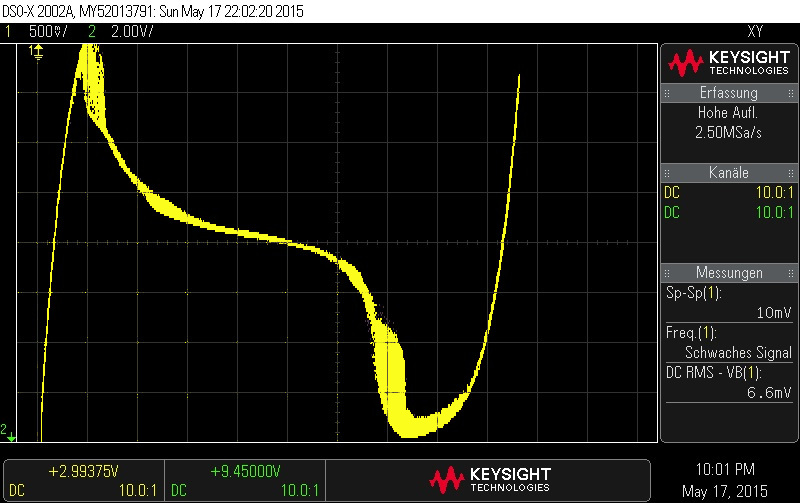
\includegraphics[width=\hsize]{tunneldiode/images/Kennlinie_DSO.jpg}
\caption{Tunneldiodenkennlinie gemessen mit dem digitalen Speicheroszilloskop
\label{tunnel:KennlinieDSO}}
\end{figure}

Ein DSO kann nur Spannungen messen. 
Um den Vorw"artsstrom durch die Diode darstellen zu k"onnen, wird ein Shuntwiderstand in Serie zur Diode geschaltet. 
Der Strom erzeugt so einen Spannungsabfall "uber dem Widerstand und kann als Spannung gemessen werden.

Die zu messenden Spannungen sind mit wenigen hundert Millivolt f"ur die Aufl"osung des DSO sehr klein. 
Um das Rauschen bei der Messung m"oglichst klein zu halten, werden die Spannungen mittels Operationsverst"arker verst"arkt. 
Die gesamte Messschaltung ist in Abbildung~\ref{tunnel:Messschaltung} ersichtlich.

\begin{figure}	%Bild Messschaltung
\centering
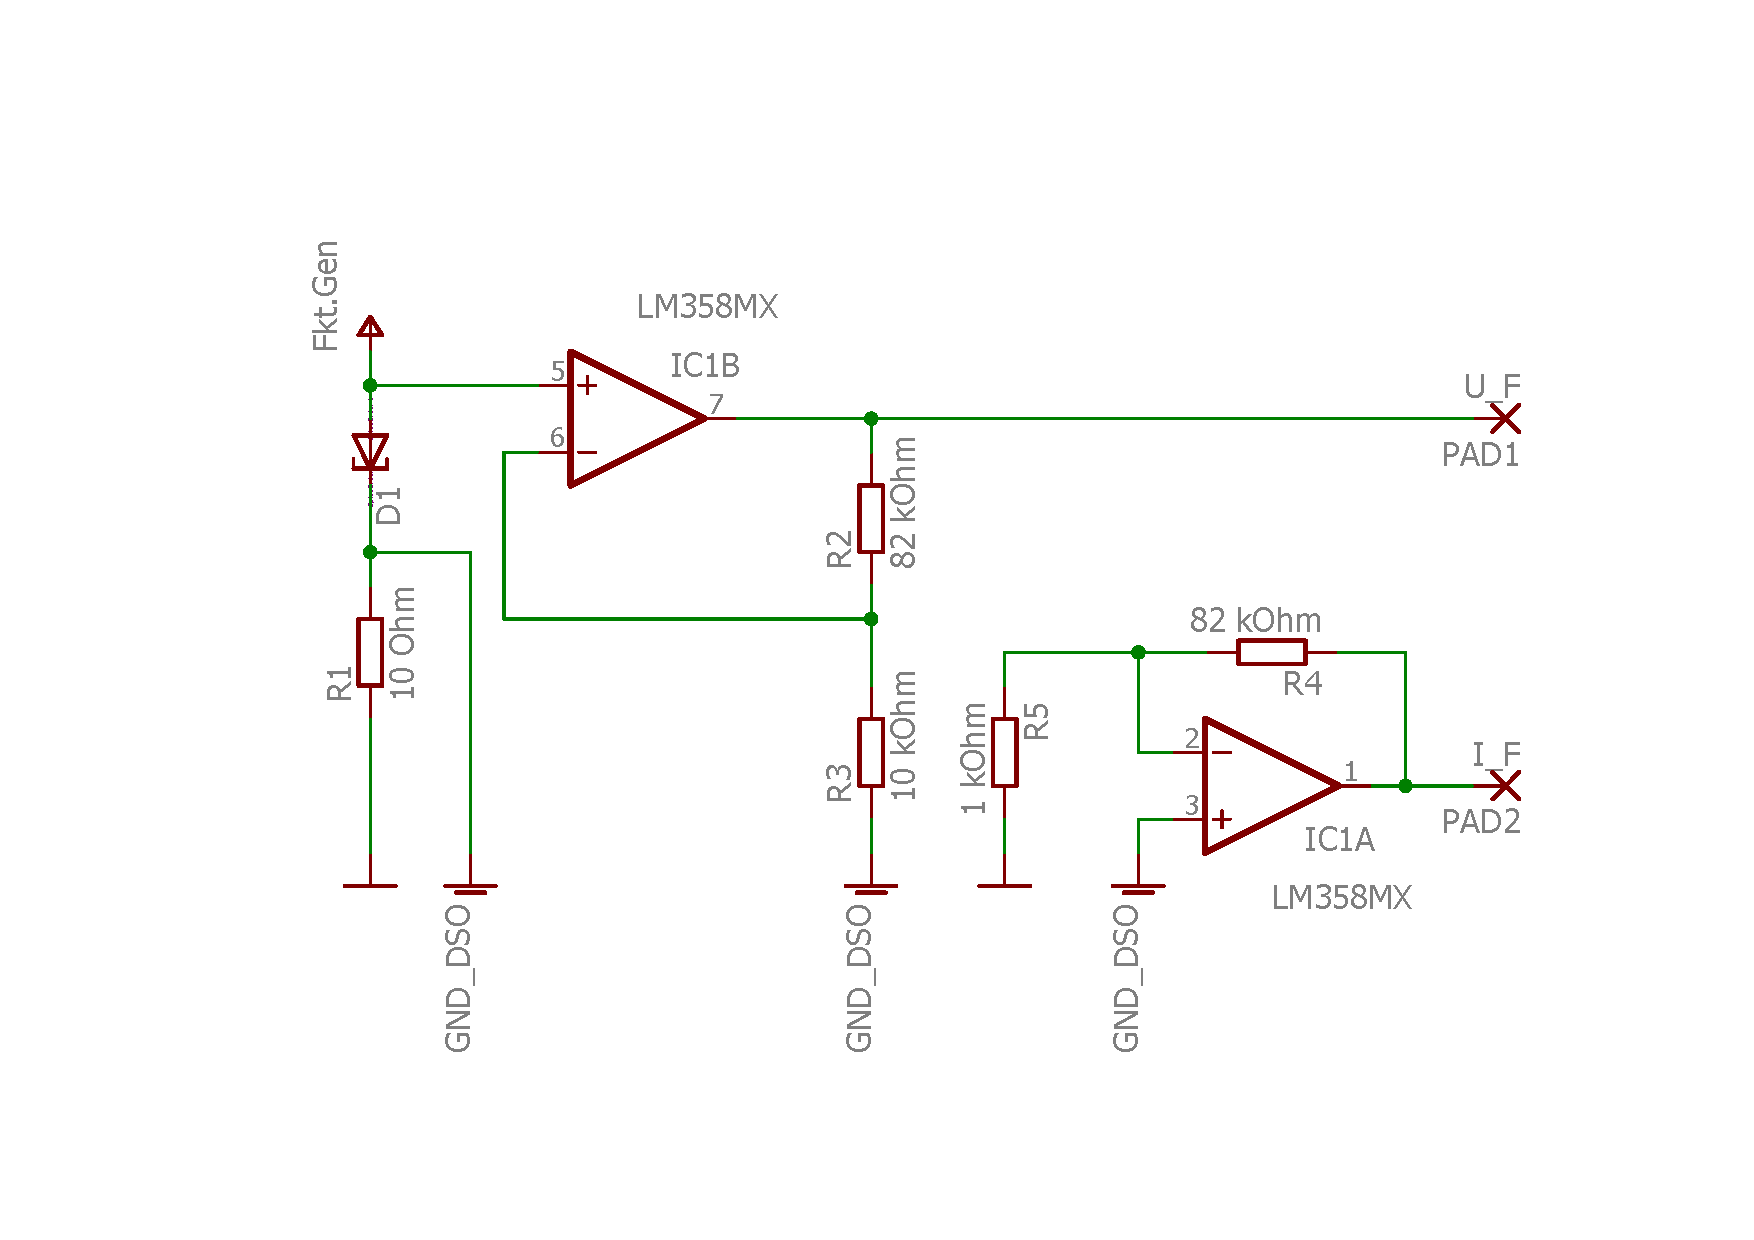
\includegraphics[width=0.7\textwidth]{tunneldiode/images/Messschaltung.pdf}
\caption{Messschaltung um die Kennlinie auszumessen
\label{tunnel:Messschaltung}}
\end{figure}

%
% Tunneldioden-Oszillator
%
% (c) 2015 Prof Dr Andreas Mueller, Hochschule Rapperswil
%
\section{Tunneldioden-Oszillator}
\rhead{Tunneldioden-Oszillator}
\begin{figure}
\centering
\includestandalone{tunneldiode/schematic}
\caption{Oszillator-Schaltung mit Tunneldiode
\label{tunnel:tunneldioden-oszillator}}
\end{figure}
Eine Tunneldiode kann dazu verwendet werden, einen Schwingkreis zu
entd"ampfen und so einen einfachen Oszillator zu konstruieren.
Eine m"ogliche Schaltung zeigt Abbildung~\ref{tunnel:tunneldioden-oszillator}.

Um die Schaltung zu analysieren, brauchen wir ein Modell f"ur die
Charakteristik der Tunneldiode. Wir nehmen dazu an, dass $U_0$ kleiner
ist also die Spannung, bei der die normale Diodenleitung einsetzt.
Dann k"onnen wir zwischen dem Strom $I_T$ durch die Tunneldiode
und der Vorw"artsspannung $U_T$ einen linearen Zusammenhang
\begin{equation}
I_T=b-aU_T
\label{tunnel:charakteristik}
\end{equation}
annehmen. $b$ entspricht in etwa dem Peak-Strom $I_{\text{peak}}$, der
Tunnelstrom bricht bei der Spannung $b/a$ zusammen.

Jetzt k"onnen wir die Differentialgleichung f"ur die Spannung $U(t)$
aufstellen. Wir bezeichnen den Spannungsabfall "uber dem Bauteil $X$
mit $U_X$ und den Strom durch das Bauteil mit $I_X$. Die Knotengleichung
bei $U(t)$ besagt:
\[
I_L+I_C=I_T
\]
Daraus und aus $U_T=U_0-U(t)$ kann $I_T$ mit Hilfe der angenommenen
Charakteristik~(\ref{tunnel:charakteristik}) der Tunneldiode eliminert werden.
Es ist
\begin{equation}
I_L+I_C=b-aU_T=b-a(U_0-U(t)).
\label{tunnel:knotengleichung}
\end{equation}
F"ur die Str"ome im Schwingkreis gilt
\begin{align*}
C\dot U_C&=I_C \qquad\text{und}\\
U_L&=L\dot I_L
\end{align*}
Nat"urlich ist $U_L=U_C=U(t)$.
Da wir in der zweiten Gleichung nur die Ableitung von $I_L$ nach
der Zeit haben, leiten wir
auch die erste und die Gleichung~(\ref{tunnel:knotengleichung}) nach
der Zeit ab, und setzen die abgeleiteten Str"ome
in~(\ref{tunnel:knotengleichung}) ein.
So erhalten wir die Differentialgleichung
\begin{equation*}
\frac1{L}U(t) +C\ddot U(t)=a\dot U(t)
\end{equation*}
oder
\begin{equation}
\ddot U(t)
-\frac{a}{C}\dot U(t)
+\frac1{LC}U(t)
=0.
\label{tunnel:dgl1}
\end{equation}
F"ur $a=0$ wird daraus eine gew"ohnliche Schwingungsdifferentialgleichung
mit Kreisfrequenz $\omega_0^2=1/LC$.

\begin{figure}
\centering
\includegraphics{tunneldiode/tunnel-8.pdf}
\caption{Designparameter $L$ und $C$ des Tunneldioden-Oszillators nach
Abbildung~\ref{tunnel:tunneldioden-oszillator}. 
Die Hyperbeln verbinden Punkte gleicher Eigenfrequenz des Schwingkreises.
Dass hellgraue Gebiet wird ausgeschlossen durch die Bedingung, dass die
Kapazit"at gross genug sein muss.
Das dunkelgraue Gebiet schliesst Werte der Induktivit"at aus, wenn die
Kreisfrequenz $\omega$ erreicht werden soll.
\label{tunnel:designparameter}}
\end{figure}

Das charakteristische Polynom der Differentialgleichung~(\ref{tunnel:dgl1})
ist
\[
\lambda^2-\frac{a}{C}\lambda +\omega_0^2\lambda=0
\]
mit den Nullstellen
\[
\lambda_\pm = \frac{a}{2C}\pm\sqrt{\frac{a^2}{4C^2}-\omega_0^2}.
\]
Damit tats"achlich Schwingungsl"osungen entstehen, muss der Radikand
negativ sein, es muss also gelten
\[
\frac{a^2}{4C^2}<\frac1{LC}
\qquad\Rightarrow\qquad
\frac{C}{L} > \frac{a^2}{4}.
\]
Die Kapazit"at $C$ muss also ausreichend gross sein.
Abbildung~\ref{tunnel:designparameter} zeigt den Raum der Design-Parameter
$C$ und $L$.

Eine grosse Kapazit"at $C$ bewirkt aber auch, dass der Koeffizient
$-a/C$ des $\dot U(t)$-Terms kleiner wird. Mit zunehmender Kapazit"at
wird als die Entd"ampfung geringer, und je nach parasit"arer D"ampfung
kann es schwierig werden, dass die Schaltung "uberhaupt anschwingt.

Die Schwingungsfrequenz wird f"ur $a\ne 0$ modifiziert zu
\begin{equation}
\omega
=
\sqrt{
\frac{1}{LC}
-
\frac{a^2}{4C^2}
}.
\label{tunnel:oszillatorfrequenz}
\end{equation}
Bei vorgegebener Schwingungsfrequenz und Induktivit"at ist dies eine
quadratische Gleichung f"ur $C$, wir schreiben sie in der gebr"auchlicheren
Form
\[
\omega^2 C^2 -\frac1{L}C+\frac{a^2}{4}=0.
\]
Diese Gleichung hat nur dann reelle L"osungen f"ur $C$, wenn die Diskriminante
positiv ist, also
\begin{equation}
\begin{aligned}
\frac1{L^2}-4\omega^2\frac{a^2}4&>0
&
&\Rightarrow&
\frac1{L^2}&>\omega^2a^2
&
&\Rightarrow&
L<&\frac1{a\omega}
\end{aligned}
\end{equation}
Wenn also die Kreisfrequenz $\omega$ angestrebt werden soll, dann darf die
Induktivit"at nicht zu gross sein.
Dies wird in Abbildung~\ref{tunnel:designparameter} durch das dunkelgraue
Gebiet dargestellt.

\begin{beispiel}
Die in diesem Kapitel genauer untersuchte Tunneldiode 1N3721 hat einen
Spitzenstrom von $I_{\text{peak}}=25\,\text{mA}$, der Tunnelstrom
bricht bei $450\,\text{mV}$ zusammen.
Wir k"onnen also von $a=25/450=0.0555\text{A/V}$ ausgehen.
Mit einer Induktivit"at von $L=0.1\mu\text{H}$ l"asst sich dann bestenfalls
die Kreisfrequenz
$\omega=1/(aL)=1/(10^{-7}\cdot 0.055)=180\cdot 10^6\,\text{s}^{-1}$
erreichen,
also die Frequenz $28.7\,\text{MHz}$.
Die Kapazit"at muss mindestens $C>La^2/4=77\text{pF}$ sein.

Mit einem $100\,\text{nF}$-Kondensator gilt f"ur die Eigenkreisfrequenz
$\omega_0$ des Schwingkreises $\omega_0^2=1/LC=10^{14}$, die Eigenfrequenz
ist also etwa $1.5915\,\text{MHz}$.
F"ur die Frequenz des Oszillators muss allerdings die
Formel~(\ref{tunnel:oszillatorfrequenz}) verwendet werden.
Da aber in unserem Fall $a^2/4\simeq 0.00077$ ziemlich klein ist, ist
die Frequenz fast gleich wie die Eigenfrequenz des Schwingkreises.
Anwendung der Formel~(\ref{tunnel:oszillatorfrequenz})
ergibt $1.5909\,\text{MHz}$, also tats"achlich nur ein sehr kleiner
Unterschied zur Eigenfrequenz.
\end{beispiel}



\section{Vermessen des Tunneldioden-Oszillators}
\rhead{Vermessen des Tunneldiode-Oszillators}

Die Grundlagen zum Tunneldioden-Oszillator werden im Abschnitt ~\ref{tunnel:oszillator} behandelt. 
Die Oszillatorschaltung wird gem"ass Abbildung ~\ref{tunnel:tunneldioden-oszillator} aufgebaut. 
F"ur den ersten Versuch wird eine Spule mit $L=100\text{nH}$ und ein Kondensator mit $C=100\text{nF}$ verwendet. 
$U(t)$ wird mit dem DSO dargestellt. 
Zus"azlich wird noch der Strom durch die Tunneldiode mit einem Multimeter gemessen. 
Die Spannung $U_0$ wird langsam erh"oht und dabei die Anzeige vom DSO beobachtet. 
Der Oszillator beginnt im Bereich vom abnehmenden Tunnelstrom zu schwingen. 
In der Abbildung~\ref{tunnel:oszi1} sieht man die Schwingung des Oszillators auf dem DSO Bildschirm. 
Die gr"osste Amplitude der Schwingung wird mit einem Tunnelstrom von etwa $I_T = 11\text{mA}$ erreicht.

\begin{figure}	%Bild Oszillator 1
\centering
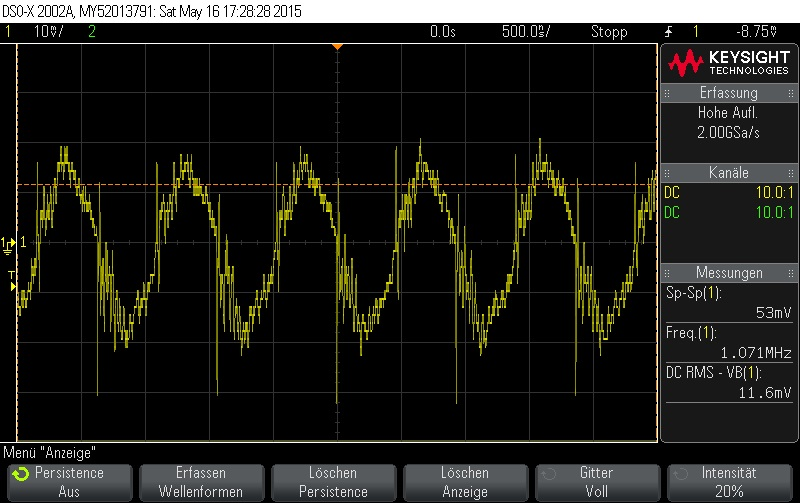
\includegraphics[width=\hsize]{tunneldiode/images/Oszi_1.jpg}
\caption{Der Tunneldioden-Oszillator schwingt mit $L = 100\text{nH}$ und $C=100\text{nF}$ bei $1.08\text{MHz}$
\label{tunnel:oszi1}}
\end{figure}

Berechnet man mit der Formel ~\ref{tunnel:oszillatorfrequenz} und den verwendeten Bauteilwerten die Kreisfrequenz $\omega$, erh"alt man eine Frequenz von $1.5909\text{MHz}$.
Die Abweichung zwischen dem gemessenen und dem berechneten Wert ist hier offensichtlich.
Ein kleiner Teil wird durch die Bauteiltoleranzen beigetragen.
Der restliche Teil wird durch das verwendete Berechnungsmodell der Tunneldiode hervorgerufen.
F"ur die Berechnung nehmen wir einfach an, dass die Tunneldiode im Bereich zwischen dem maximalen Tunnelstrom und der normalen Diodenleitung eine lineare Kennlinie hat.
Schauen wir uns nochmals die Abbildung~\ref{tunnel:Tunneldiode} an.
Da sehen wir, dass die Kennlinie alles andere als linear ist in diesem Bereich.
Wenn wir jetzt die Formel ~\ref{tunnel:oszillatorfrequenz} nach $a$ umstellen und ausrechnen, erhalten wir den Wert $a = 1.55591\text{A/V}$.
Die Steigung bei diesem Arbeitspunkt ist also sehr viel gr"osser als die gemittelte Steigung "uber den gesamten abfallenden Teil.

Versuchsweise wird die Spule durch eine um Faktor 10 gr"ossere ersetzt. 
Die Induktivit"at ist somit $L=1\mu\text{H}$. 
Die Frequenz muss mit der gr"osseren Spule kleiner werden. 
In der Abbildung~\ref{tunnel:oszi2} kann man sehen, dass sich die Frequenz etwa halbiert.
Rechnet man jetzt hier ebenfalls mit der Formel ~\ref{tunnel:oszillatorfrequenz} die Kreisfrequenz $\omega$, erh"alt man eine Frequenz von $501.351\text{kHz}$.
Die Berechnung stimmt ziemlich genau mit der Messung "uberein.
Je nachdem wo der DC-Arbeitspunkt liegt, kann das lineare Modell f"ur die Tunneldiode verwendet werden.

\begin{figure}	%Bild Oszillator 2
\centering
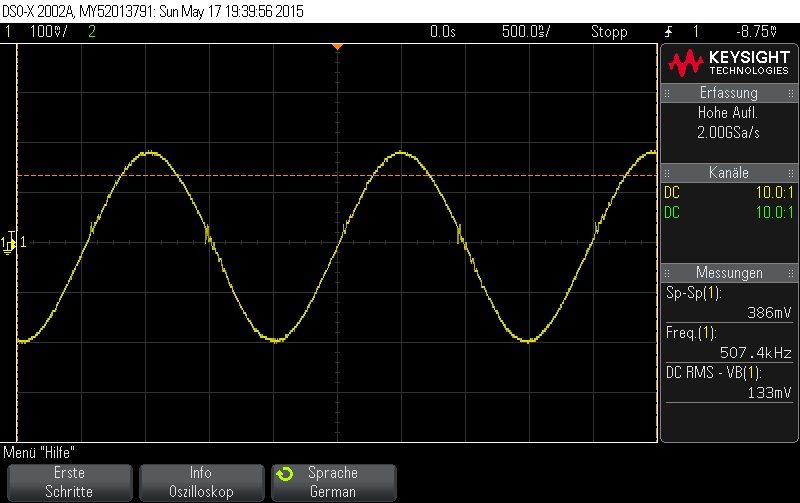
\includegraphics[width=\hsize]{tunneldiode/images/Oszi_2.jpg}
\caption{Der Tunneldioden-Oszillator schwingt mit $L = 1\mu\text{H}$ und $C=100\text{nF}$ bei $507\text{kHz}$
\label{tunnel:oszi2}}
\end{figure}

\section{Fazit}
\rhead{Fazit}
Obwohl die Tunneldiode in der heutigen Zeit fast vollst"andig durch andere Bauelemente ersetzt worden ist, war sie mal ein wichtiges Bauteil in der HF-Technik.
In Oszillatoren wurden mit der Tunneldiode Frequenzen bis zu $100\text{GHz}$ erreicht.
Sie wurde neben der Verwendung in Oszillatoren auch als Schalter f"ur schnelle Signale bis zu $10\text{GHz}$ eingesetzt.

\printbibliography[heading=subbibliography]
\end{refsection}

